% Rappresenta il tipo di documento
\documentclass[12pt, twoside]{book}

% Elenco dei packages utilizzati
\usepackage[a4paper,width=150mm,top=25mm,bottom=25mm,bindingoffset=6mm]{geometry}
\usepackage[utf8]{inputenc}
\usepackage[T1]{fontenc}
\usepackage[italian]{babel}
\usepackage{subcaption}
\usepackage{graphicx}
\usepackage{fancyhdr}
\usepackage{float}
\usepackage{color}
\usepackage[nottoc]{tocbibind}
\usepackage{emptypage}
\usepackage[hidelinks]{hyperref}
\usepackage{titlesec}
\usepackage{amssymb}
\usepackage[sorting=none,backend=bibtex]{biblatex}
\usepackage{csquotes}
\usepackage{pdfpages}
\usepackage{amsmath}
\usepackage{placeins}
\usepackage{hyperref}
\usepackage{footnote}
\usepackage{minted}
\usepackage{xcolor}

% Stile di pagina
\pagestyle{fancy}
\definecolor{LightGray}{gray}{0.9}
\usemintedstyle{colorful}

\renewcommand{\chaptermark}[1]{\markboth{#1}{}}
\renewcommand{\tocetcmark}[1]{\markboth{#1}{}}
\renewcommand{\sectionmark}[1]{\markright{\thesection\ #1}}
\fancyhf{}
\fancyhead[LE,RO]{\bfseries\thepage}
\fancyhead[LO]{\bfseries\rightmark}
\fancyhead[RE]{\bfseries\leftmark}
\renewcommand{\headrulewidth}{0.5pt}
\fancypagestyle{plain}{
    \fancyhead{}
    \renewcommand{\headrulewidth}{0pt}
}
\setlength{\headheight}{28pt}

% Stile dei titoli dei capitoli
\definecolor{gray75}{gray}{0.75}
\newcommand{\hsp}{\hspace{20pt}}
\titleformat{\chapter}[hang]
{\Huge\bfseries}
{\thechapter\hsp\textcolor{gray75}{|}\hsp}
{0pt}
{\Huge\bfseries}

% Impostazioni bibliografia
\addbibresource{./bibliografia/bibliografia.bib}

% Ridefinizione enfasi
%\DeclareTextFontCommand{\emph}{\bfseries\em}

% Inizio del documento
\begin{document}

% Frontespizio

\includepdf{./frontespizio/frontespizio.pdf}

\cleardoublepage
\begin{flushright}
\thispagestyle{empty}
\null\vspace{\stretch {1}}
\textit{Dedica dedicosa.\break --- A capo.}
\vspace{\stretch{2}}\null
\end{flushright}
\cleardoublepage

% Indice
\tableofcontents

% Elenco delle figure
\phantomsection
\listoffigures

% Introduzione
\chapter*{Introduzione}
\chaptermark{Introduzione}
\addcontentsline{toc}{chapter}{Introduzione}
La sicurezza informatica risulta importante per la salvaguardia dei dati personali. In particolare, è necessario assicurare i seguenti due aspetti:
\begin{itemize}
    \item \textbf{Confidenzialità:} la garanzia per la quale un utente non autorizzato non possa accedere a informazione riservate.
    \item \textbf{Integrità:} la garanzia per la quale un utente non autorizzato non possa modificare informazioni e dati personali.
\end{itemize}
Esistono diversi meccanismi di autenticazione, divisi tra:
\begin{itemize}
    \item ``Cosa si possiede'': oggetti fisici fini all'autenticazione, tra i quali chiavi, badge elettronici, token fisici, ecc.
    \item ``Cosa si è'': identificazione tramite caratteristiche fisiche, tra cui il riconoscimento facciale, l'impronta digitale, scansione dell'iride.
    \item ``Cosa si sa'': sequenze alfanumeriche che compongono una password o un PIN, informazioni personali private.
\end{itemize}
In questo documento si pone maggiore attenzione alla generazione di parole chiave, poiché risulta il meccanismo maggiormente utilizzato e facilmente raggirabile. Esistono diverse tecniche di attacco che compromettono la sicurezza che una password solitamente offre, come ad esempio gli attacchi a forza bruta che tentano tutte le possibili combinazioni di caratteri, oppure gli attacchi a dizionario che utilizzano un corpus di parole.

Le strategie di attacco possono essere di due tipologie in base a se si possiedono dati riguardanti un determinato utente: mirato, nel caso in cui si disponga di informazioni personali riguardanti l'utente e ottenute tramite ingegneria sociale o leak di dati, non mirato altrimenti.

In seguito alla creazione di molteplici profili da parte di un utente e violazioni di dati personali è spesso riscontrata la tendenza di riutilizzare la stessa password ~\cite{google} o varianti di essa. Ciò può comportare la compromissione della propria identità e pericoli relativi alla privacy online.

In questo lavoro di tesi vengono analizzati i pericoli relativi al fenomeno di password reuse, e proposti approcci di prevenzione, che sfruttano tecniche di machine learning basati su lavori presenti in letteratura~\cite{bijeeta}.

Si cercherà in particolare di approfondire l'approccio utilizzato, in modo da potere proporre migliori strategie fini alla analisi della similarità tra password.

% Capitoli
\chapter{Stato dell'arte}
\label{ch:state of the art}

La sicurezza delle password al giorno d'oggi riveste un ruolo significativo nel garantire confidenzialità e integrità dei dati personali degli utenti e delle aziende.
Solitamente si è più propensi a scegliere password semplici da ricordare, come riferimenti autobiografici, oppure sequenze di caratteri molto comuni (e.g. \texttt{qwerty}, \texttt{123456}).
Per semplificare la memorizzazione, si utilizzano spesso password brevi, in media da 9-10 caratteri e composte in gran parte da caratteri minuscoli~\cite{obspasshab}.

Tuttavia questa scelta porta a maggiori probabilità di subire violazioni dei propri account, poiché password semplici sono vulnerabili ad attacchi di forza bruta. Inoltre, tramite tecniche di ingegneria sociale, è possibile individuare il criterio di scelta dell'utente, eventualmente ragionando sui dati disponibili grazie ai data breach.

Nel 2020 sono stati confermati 3950 data breach, dal costo medio di 3,86 milioni di dollari. Il 52\% dei breach è stato causato da attacchi informatici e il numero di giorni medio per individuare un breach è stato di 207 giorni~\cite{ibmcost}.
Il 42\% è causato da attacchi su applicazioni web e il metodo più comune di attacco (82\%) ha utilizzato credenziali rubate o ottenute tramite attacchi a forza bruta.
Il 58\% dei breach conteneva dati personali~\cite{verizon}.
\begin{figure}[h]
    \centering
    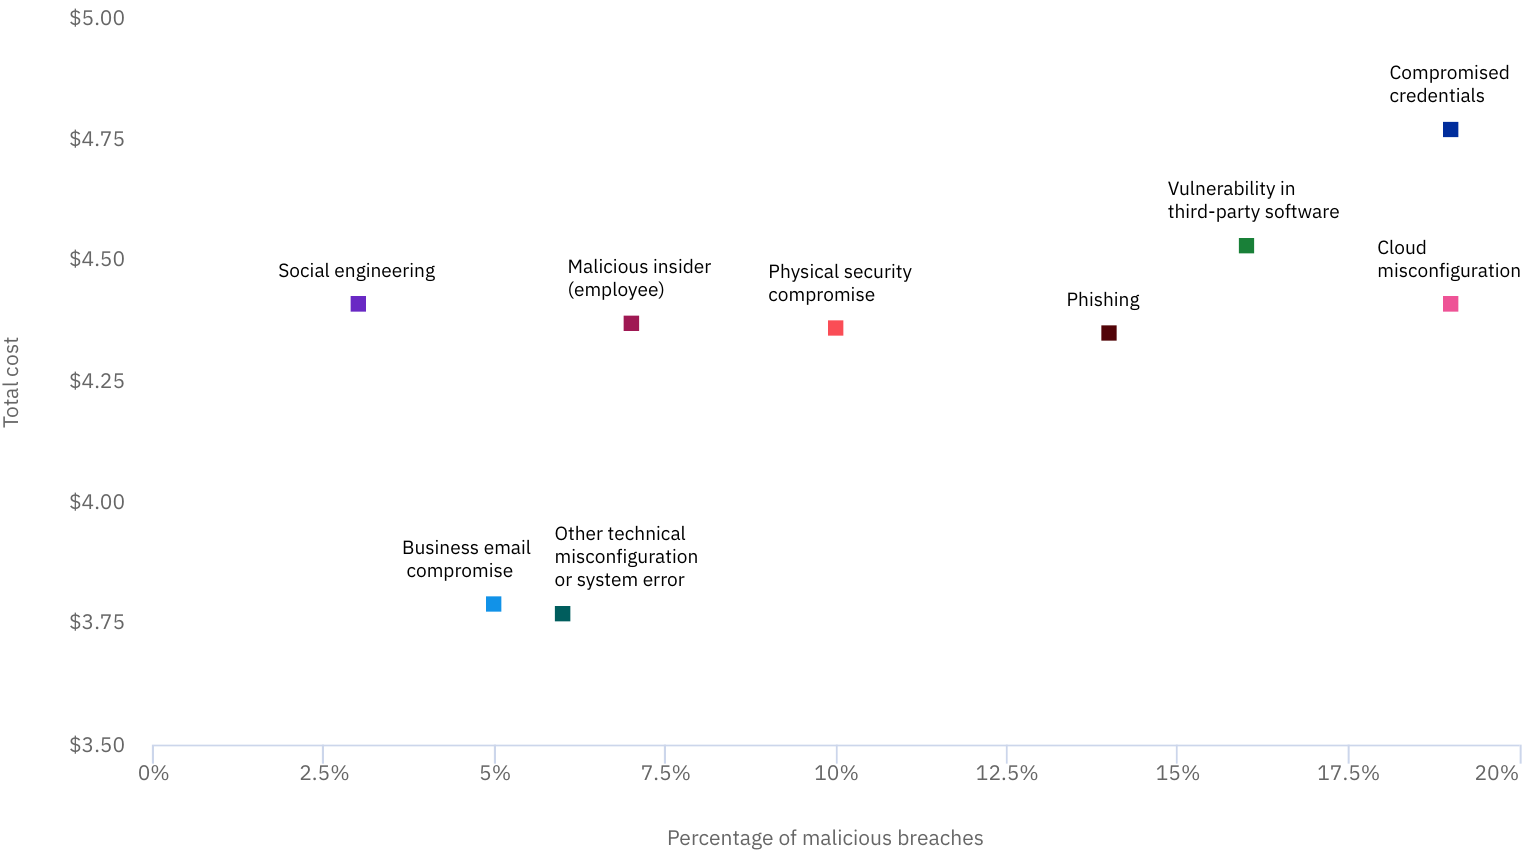
\includegraphics[width=15cm]{./immagini/prova.png}
    \label{data breach}
    \caption{Costo medio e frequenza di data breach causati da attacchi informatici, in base alla causa, nel 2020~\cite{ibmcost}}
\end{figure}

Sebbene la maggior parte delle password siano crittografate, è possibile risalire alla forma testuale mediante strumenti come Hashcat\footnote{\url{https://github.com/hashcat/hashcat}} e John The Ripper\footnote{\url{https://github.com/openwall/john}}.

In seguito alla diffusione delle credenziali, gli utenti decidono di cambiare password e la scelta ricade spesso su varianti usate su altri account.
\section{Scelta di una nuova password}
\label{sec:scelta di una nuova password}
L'utente medio ha la tendenza a scegliere password semplici~\cite{obspasshab}. Per questo motivo, spesso la nuova password è il risultato di una leggera variazione della vecchia password, o una combinazione di password precedenti~\cite{hypr}.

Un modo per verificare la sicurezza della password è utilizzare strumenti come zxcvbn\footnote{\url{https://github.com/dropbox/zxcvbn}}, che riesce a riconoscere:
\begin{itemize}
    \item 30000 password comuni;
    \item nomi e cognomi comuni negli USA;
    \item parole spesso utilizzate in inglese su Wikipedia;
    \item parole spesso utilizzate alla televisione e film statunitensi;
    \item date;
    \item ripetizioni di lettere (\texttt{aaaa});
    \item sequenze alfabetiche (\texttt{abcde});
    \item sequenze di tastiera (\texttt{qwertyuiop});
    \item il codice \texttt{l33t}.
\end{itemize}

Altri strumenti, come Kaspersky password checker\footnote{\url{https://password.kaspersky.com/it/}}, controllano anche dati di numerosi data breach raccolti da Have I been Pwned?\footnote{\url{https://haveibeenpwned.com/}}.
Questi approcci, tuttavia, non controllano la cronologia delle password di uno specifico utente, ma soltanto la resistenza ad attacchi di forza bruta.

Per questo motivo sono state studiate strategie che tengono conto delle credenziali utilizzate.
Alcune sfruttano un approccio probabilistico, come i \emph{Bloom filter}~\cite{bloom}. Un'altra possibile modalità utilizza \emph{word embedding} di password.

\section{Word embedding}
\label{sec:word embedding}
Per capire il contesto delle parole e per poterle rappresentare in base alla sfera semantica e alla sintassi, si ricorre un insieme di tecniche che prevedono il mapping delle parole o delle frasi di un dizionario in vettori di numeri reali, note come \emph{word embedding}.
Parole simili possiedono una codifica simile.


Per stabilire il valore di ogni embedding si allena una rete neurale con specifici parametri e le dimensioni variano tra 8 (per piccoli dataset) a 1024. Maggiore è la dimensione di un embedding, maggiore risulta la quantità di informazioni relativa alle relazioni tra parole~\cite{tensword}.

\subsection{Similarità tra parole}
\label{Similarita tra parole}
Per potere stabilire se due parole appartengono alla stessa sfera semantica si utilizza un metodo noto come \emph{cosine similarity}.
\begin{equation}
    similarity = cos(\theta) = \frac{A\cdot{B}}{\|A\|\cdot{\|B\|}}
\end{equation}

Due parole risultano simili quando il valore del coseno è 1, ovvero quando l'angolo tra i due vettori risulta nullo. Si consideri il seguente esempio:

\begin{figure}[h]
    \centering
    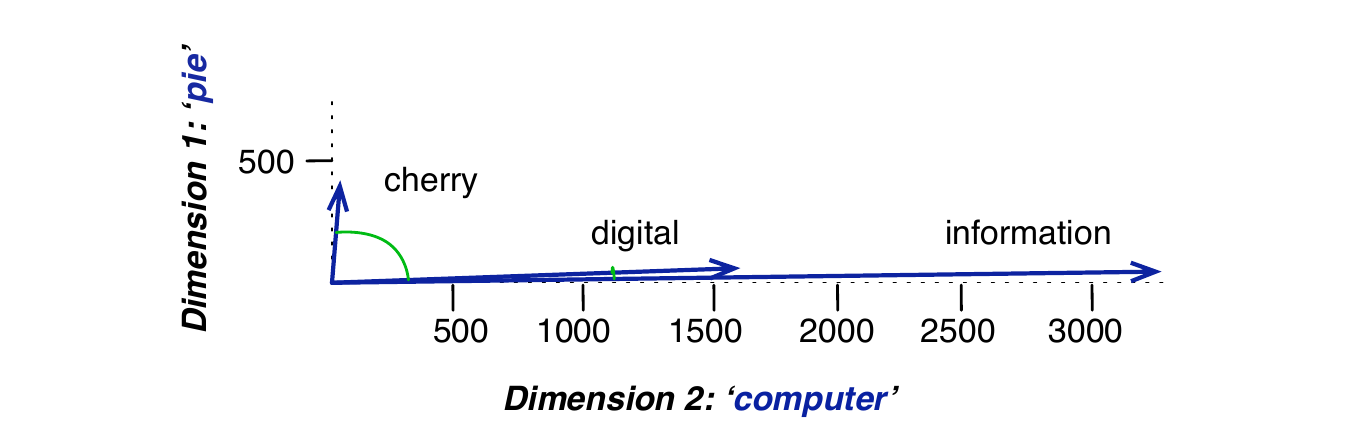
\includegraphics[width=11cm]{./immagini/cosine_similarity_esempio.png}
    \label{cosine}
    \caption{Esempio di calcolo della similarità tra word embedding~\cite{cosine}}
\end{figure}

Nella figura sono mostrati i vettori di 3 parole (\textit{cherry}, \textit{digital} e \textit{information}) in uno spazio bidimensionale definiti dal numero di occorrenze in vicinanza alle parole \textit{computer} e \textit{pie}.
Come si può notare, l'angolo tra \textit{digital} e \textit{information} risulta minore rispetto all'angolo tra \textit{cherry} e \textit{information}.
Quando due vettori risultano più simili tra loro, il valore del coseno risulta maggiore, ma l'angolo risulta minore. Il coseno assume valore massimo 1 quando l'angolo tra i due vettori risulta nullo (0°); il coseno degli altri angoli risulta inferiore a 1~\cite{cosine}.
\subsection{Tipologie di word embedding}
\label{sec:tipologie di word embedding}
\subsubsection{Word2Vec}
\label{sec:word2vec}
Word2Vec è un insieme di modelli architetturali e di ottimizzazione utilizzati per imparare word embedding da un vasto corpus di dati, sfruttando reti neurali.
\\
Un modello allenato con Word2Vec riesce a individuare le parole simili tra loro, in base al contesto, grazie alla \textit{cosine similarity} esaminata precededentemente.

\begin{figure}[h]
    \centering
    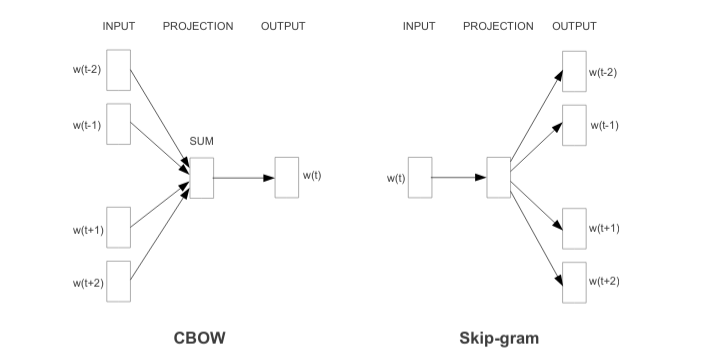
\includegraphics[width=15cm]{./immagini/cbow_vs_skipgram.png}
    \label{cbowskipgram}
    \caption{CBOW vs skip-gram~\cite{mikolov2013efficient}}
\end{figure}
\newpage
Word2Vec utilizza due modelli di architetture:
\begin{itemize}
    \item \textbf{CBOW} (continuous bag of words): l'obiettivo del training è combinare le rappresentazioni delle parole limitrofe per prevedere la parola centrale.
    \item \textbf{Skip-gram}: simile a CBOW, con la differenza che viene utilizzata la parola centrale per prevedere le parole circostanti relative allo stesso contesto\cite{fasttext}.
\end{itemize}

CBOW risulta più veloce ed efficace in caso di dataset di grandi dimensioni, tuttavia, nonostante la maggiore complessità, Skip-gram è in grado di trovare parole non presenti nel corpus, per dataset di minori dimensioni~\cite{mikolov2013efficient}.


\subsubsection{FastText}
\label{sec:fasttext}
FastText è una libreria open-source proposta da Facebook che estende Word2Vec, e consente un apprendimento efficiente di rappresentazioni di parole e di classificazioni di frasi.
Anziché allenare un modello fornendo ogni singola parola di un dataset, FastText prevede l'apprendimento tramite \textit{n-gram} di ciascuna parola.

Si definiscono n-gram di una parola costituita da $c_1...c_m$ caratteri la seguente sequenza:
\begin{center}
$\{ c_{i_1}, c_{i_2}, \ldots, c_{i_n} \mid \sum\limits_{j=1}^n i_{j} - i_{j-1} < 0 \}$
\end{center}
Ad esempio, gli n-gram della parola ciao, con $n\_mingram = 1$ e $n\_maxgram = 4$, sono i seguenti:
%Si considerino gli n-gram della parola $ciao$:

\begin{center}
    $ciao = \{\{c, i, a, o\},\{ci, ia, ao\}, \{cia, iao\}, \{ciao\}\}$
\end{center}
$ciao$ viene espresso come l'insieme di tutte le sottostringhe di lunghezza minima pari a 1, e lunghezza massima pari a 4.

%In questo esempio, con $n\_mingram = 1$ e $n\_maxgram = 4$, $ciao$ viene espresso come l'insieme di tutte le sottostringhe di lunghezza minima pari a 1, e lunghezza massima pari a 4.


FastText consente di ottenere, con più probabilità rispetto a Word2Vec, parole \emph{out-of-dictionary}, ovvero parole sconosciute al modello in fase di training.
\chapter{Analisi progettuale}
\label{ch:analisi progettuale}

In questo progetto si cerca di sviluppare un sistema per verificare in modo robusto la similarità tra password di un utente, in modo da evitare di utilizzare varianti di password precedenti, e garantire maggiore sicurezza di uno o più account.
A tal proposito sono stati condotti esperimenti che, per controllare la similarità tra password, utilizzavano word embedding di parole. In questo lavoro di tesi è stato preso come riferimento il paper di Bijeeta  et alii~\cite{bijeeta}.

\section{Modelli di similarità tra password basati sulle reti neurali}
\label{sec:modelli di similarita tra password basati sulle reti neurali}
Solitamente le metriche che misurano la robustezza di password non tengono conto della cronologia delle password passate di un utente.
Ciò può costituire un problema sia se si effettua un attacco contro un utente, sia per proteggerlo:
\begin{itemize}
    \item Durante un attacco, si considerano determinate password note grazie a leak, tuttavia non è presente un approccio flessibile che elabori varianti di password di un determinato utente.
    \item Non è presente un meccanismo che avverta l'utente del potenziale pericolo causato dal riutilizzo di password.
\end{itemize}
Per questo motivo, nel paper riferimento di Bijeeta et alii~\cite{bijeeta} sono stati utilizzate due tipologie di reti neurali:
\begin{itemize}
    \item Per l'attacco è stato sviluppato un modello di rete neurale ricorrente, noto come pass2path.
    \item Per la difesa sono stati utilizzate tecniche di Natural Language Processing, in particolare modelli di word embedding, i quali generano una corrispondenza tra parole e vettori, mantenendo proprietà semantiche della password originale, come la similarità.
\end{itemize}

\section{Prerequisiti}
\label{sec:prerequisiti}
Per la creazione dei due modelli visti precedentemente, è stato utilizzato un leak disponibile sul Deep Web, di dimensione pari a 45 GB e contenente 1.4 miliardi di coppie mail-password appartenenti ad account su social come LinkedIn, MySpace, Badoo, Yahoo, Zoosk; successivamente è stato filtrato nel seguente modo:

\begin{itemize}
    \item sono state rimosse le stringhe che contenevano 20 o più caratteri esadecimali;
    \item sono stati rimossi hash non decodificati;
    \item sono state rimosse le password più lunghe di 50 caratteri o più corte di 3 che contenevano caratteri non ASCII;
    \item sono stati rimossi 4528 utenti associati a centinaia di password, poiché è molto improbabile che siano account veri.
\end{itemize}

Dal risultato del processo di filtraggio sono stati osservati i seguenti punti:
\begin{itemize}
    \item la password 123456 è stata utilizzata dal 0.9\% degli utenti;
    \item più dell'88\% di password hanno una lunghezza compresa tra 6 e 12 caratteri;
    \item l'80\% delle password contiene solo caratteri minuscoli.
\end{itemize}

\begin{figure}[h]
    \centering
    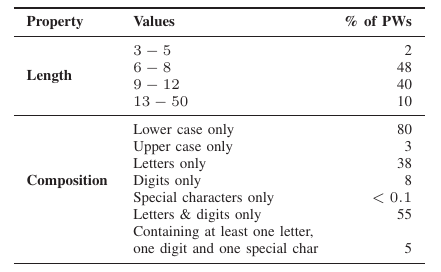
\includegraphics[width=11cm]{./immagini/pulizia_dataset_bijeeta.png}
    \label{pulizia dataset}
    \caption{La distribuzione della lunghezza delle password e della loro composizione dopo la pulizia del dataset~\cite{bijeeta}}
\end{figure}



\section{Strategie di attacco: pass2path}
\label{sec:pass2path}
\subsection{Euristiche e appartentenza di password}
\label{sec:euristiche e appartenenza di password}
Una volta ottenuto il dataset, è necessario capire a quali persone appartengono gli account. A tal proposito vengono proposte tre euristiche:
\begin{itemize}
    \item \textbf{Basata su email:} gli utenti vengono identificati solo dalla email. Ciascuna email appartiene a un solo utente.
    \item \textbf{Basata sugli username:} si considera la stringa che precede \texttt{@} nell'indirizzo email. Un utente può possedere più mail, tutte identificate dalla stringa che precede \texttt{@}.
    \item \textbf{Basata su un metodo misto:} considera sia gli username che le email. Due email sono considerate connesse tra loro se hanno almeno una password in comune e se le mail connesse tra loro sono associate allo stesso username.
\end{itemize}
Per potere effettuare migliori test sul dataset sono stati rimossi gli utenti che avevano meno di due password associate allo stesso account.

Il dataset successivamente viene diviso in due parti: training set e test set (in rapporto 80\%-20\% ). Nel paper la fase di training utilizza soltanto il dataset relativo all'euristica basata sulle email, mentre per la fase di testing si utilizza sia l'euristica basata sulle email sia quella mista.

\subsection{Introduzione a pass2path}
\label{sec:intro pass2path}
Pass2path è un modello di rete neurale che consente di creare password in grado di compromettere più del 48\% degli utenti in meno di mille tentativi. Il successo di questo modello è dovuto al riutilizzo della stessa password o di varianti di password da parte dell'utente.
Per svilupparlo si è tenuto conto della sequenza di trasformazioni $\tau_1...\tau_n $, nota come \emph{percorso} che consente, a partire dalla password  $\tilde{w}$, di produrre la nuova password $w$.


Le modifiche sono rappresentate da una unità di misura $\tau\in \mathcal{T}$, che specifica in che posizione e quale tipo di variazione applicare a una password.
\\
$\tau$ è composto da una tripletta  $\{e, c', l\}$:
\begin{itemize}
    \item $e$ rappresenta una modifica da apportare;
    \item $c'$ rappresenta un carattere o una stringa vuota;
    \item $l$ rappresenta la posizione della modifica della password.
\end{itemize}

Le modifiche vengono classificate in tre tipologie:
\begin{itemize}
    \item \texttt{sub} (sostituzione);
    \item \texttt{ins} (inserimento);
    \item \texttt{del} (cancellazione).
\end{itemize}

Se si considera $c'$ sono presenti due situazioni:
\begin{itemize}
    \item \texttt{ins} e \texttt{sub}: $c'$ rappresenta il carattere o la stringa vuota;
    \item \texttt{del}: è sempre una stringa vuota.
\end{itemize}

Per ricavare il percorso tra due password, si considera quello più corto, nel seguente ordine decrescente di preferenza:
\begin{enumerate}
    \item \texttt{del};
    \item \texttt{ins};
    \item \texttt{sub}.
\end{enumerate}

Le varie trasformazioni del percorso vengono ordinate in base alla posizione della modifica.

Ad esempio, il percorso da \texttt{cats} a \texttt{kates} (distanza di modifica pari a 2) è:
\begin{center}
    $path = \{(sub , k^\prime , 0), (ins , e^\prime , 3)\}$
\end{center}

\subsection{Come allenare pass2path}
\label{sec:allenamento pass2path}
Prima di allenare pass2path è necessario tradurre ciascuna password come sequenza di tasti premuti su una \emph{tastiera americana ANSI}. La codifica dei tasti premuti è la seguente:
\begin{itemize}
    \item Per rappresentare una sola lettera maiuscola all'interno di una parola si pone \texttt{<s>} (che rappresenta la pressione del tasto \texttt{SHIFT}) prima della lettera, che viene lasciata minuscola. Ad esempio \texttt{Ciao} viene tradotto come \texttt{<s>ciao}.
    \item se si hanno più lettere maiuscole consecutive seguite da lettere minuscole si pone \texttt{<c>} (che rappresenta la pressione del tasto \texttt{CAPS LOCK}) prima e dopo la sequenza di lettere maiuscole, che viene lasciata minuscola. Per esempio \texttt{PASSword} viene tradotto come \texttt{<c>pass<c>word}.
    \item Nel caso di una sequenza di lettere maiuscole che si conclude alla fine della parola basta porre \texttt{<c>} all'inizio della sequenza. Per esempio \texttt{PASSWORD} viene tradotto come \texttt{<c>password} e \texttt{passWORD} come \texttt{pass<c>word}.
    \item Se si hanno caratteri speciali ASCII 128 si pone \texttt{<s>} davanti al carattere.
    \\
    Quest'ultimo viene tradotto come il tasto che viene premuto insieme a \texttt{SHIFT}.
    Per esempio \texttt{PASSWORD!} viene rappresentata come \texttt{<c>password<s>1}, dato che \texttt{1} viene premuto insieme a \texttt{SHIFT} e \texttt{Hello@!!} viene tradotto come
    \\
    \texttt{<s>hello<s>2<s>1<s>1}.
\end{itemize}

\begin{figure}[h]
    \centering
    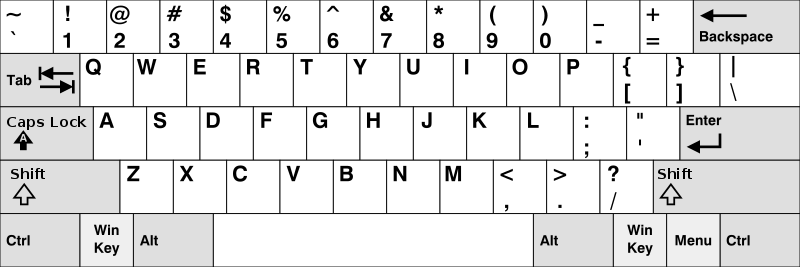
\includegraphics[width=15cm]{./immagini/US_keyboard_layout.png}
    \label{US layout}
    \caption{\href{https://upload.wikimedia.org/wikipedia/commons/thumb/5/51/KB_United_States-NoAltGr.svg/800px-KB_United_States-NoAltGr.svg.png}{Layout della tastiera americana ANSI, fonte: Wikipedia}}
\end{figure}

Successivamente occorre trovare il percorso di transizioni  $\tau_1...\tau_n$ che consentano di trasformare la password $\tilde{w}$ in $w$.

Si è deciso di filtrare le password in base alla lunghezza del percorso, che deve tenere conto anche della modifica di una password basata sulla sequenza di tasti premuti. Sono state eliminate le password con un percorso di lunghezza superiore a $\delta$.

Per allenare pass2path si utilizza il dataset di training basato sulle email.
Si utilizzano due reti neurali ricorrenti (RNN) per costruire un auto-encoder~\cite{Sherstinsky_2020}.

\subsection{Efficacia d'attacco con configurazioni non ripetute}
\label{sec:attacco conf non ripetute}
Per verificare l'efficacia di attacco della rete si utilizza il dataset di test delle email, con password da indovinare $w$ diverse dalla originale $\tilde{w}$.
Con configurazioni non ripetute, pass2path riesce in meno di 100 stime a ricavare
il 13\% delle password, impiegando 4 ore in tutto (Intel i9 e 128 GB di RAM, su un singolo thread).
\begin{figure}[h]
    \centering
    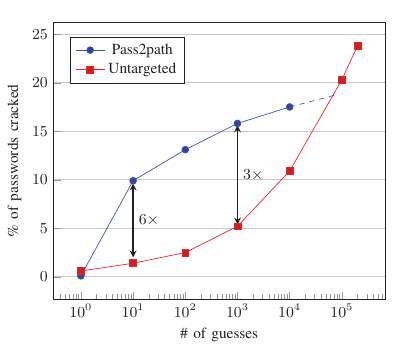
\includegraphics[width=10cm]{./immagini/pass2path.png}
    \label{pass2path}
    \caption{Pass2path riesce a indovinare in meno di mille tentativi una percentuale più alta di password, rispetto ad attacchi non mirati. Questi ultimi risultano efficaci soltanto se sono richiesti più di 1000 tentativi~\cite{bijeeta}}
\end{figure}

\subsection{Efficacia d'attacco con configurazioni ripetute}
\label{sec:attacco conf ripetute}
Per verificare l'efficacia di un attacco della rete, in caso di password da indovinare $w$ simile alla originale $\tilde{w}$, si utilizza il test set del dataset misto, in cui si è osservato che il 40\% delle password vengono riutilizzate dagli utenti, rendendoli facili bersagli.

Come primo attacco viene utilizzata la password $\tilde{w}$, in modo da verificare il suo riutilizzo senza varianti, mentre i restanti $q - 1$ vengono svolti in accordo alla tecnica di attacco scelta. Confrontando con altri modelli utilizzati, il migliore risultato è stato ottenuto da pass2path, compromettendo metà degli utenti (48.3\%) in al massimo mille tentativi.
Si è osservato che con password riutilizzate, aumentano le probabilità di indovinare la password con pass2path.
Inoltre è importante sottolineare che gli attacchi di tipo non mirato (untargeted) ottengono migliori performance se vengono eseguiti più di 1000 tentativi; al contrario pass2path è il migliore approccio nel caso in cui si proceda con un numero minore.


I ricercatori hanno anche eseguito un vero e proprio attacco all'interno della loro università (Cornell University), in modo da potere testare su password diverse da quelle del dataset, ovvero appartenenti a studenti e professori. Il migliore risultato è stato ottenuto da pass2path, che in meno di 1000 tentativi è riuscito a scoprire la password del 8,4\% degli account~\cite{bijeeta}.


\section{Difesa}
\label{sec:difesa}
\subsection{Difesa da attacchi a dizionario mirati}
\label{sec:difesa attacchi mirati}
Diversi studi mostrano che cambiare password non protegge completamente un utente dagli attacchi~\cite{google}~\cite{hypr}.
Nel paper viene illustrato il concetto di PPSM (Personalized password strength meters), che sfruttano modelli preallenati di word embedding per dimostrare la sicurezza di una password.
In questo modo si possono prevenire attacchi che sfruttano varianti di password presenti in data breach.

\subsection{Personalized password strength meters}
\label{sec:ppsm}
Un PPSM può essere utilizzato con lo scopo di dare un giudizio in tempo reale all'utente sulla sicurezza delle password durante la selezione.
Il funzionamento è il seguente:
\begin{itemize}
    \item vengono considerati in input una potenziale password e un set di password associate all'utente trovate in un data leak;
    \item vengono utilizzati due possibili criteri come output:
    \begin{itemize}
        \item \textbf{guess rank}, ovvero il numero di tentativi di una tipologia di attacco fatti prima di indovinare la password;
        \item \textbf{percentuale di similarità}, ovvero la somiglianza tra la potenziale password e la password associata all'utente.
    \end{itemize}
\end{itemize}

Un possibile modo di ottenere il guess rank è basarsi su pass2path, in modo da evitare che un utente usi una password simile a quella trovata in un data breach; tuttavia prevedere password risulta costoso (dato che si considera un modello di generazione di password come pass2path) e, nel caso in cui si vogliano inviare i risultati via rete, viene occupata molta banda.

Si è osservato che risulta più efficiente e meno costoso assegnare punteggi che rappresentano la sicurezza di una password rispetto ai guess rank~\cite{bijeeta}.

\subsection{Realizzazione di un PPSM}
\label{sec:realizzazione ppsm}
Sotto al PPSM si trova un classificatore binario $C$ che prende in input una password candidata $w$ e una password nota da un leak $\tilde{w}$ e restituisce 0 se $w$ è indovinabile in meno di 1000 tentativi a partire da $\tilde{w}$, 1 altrimenti.
Per costruire tale classificatore è necessario utilizzare tecniche di word-embedding.

\subsection{Similarità tra password via word embedding}
\label{sec:similarita via word embedding}
Si definisce word embedding la tecnica di mappatura di un insieme di parole in uno spazio vettoriale d-dimensionale (solitamente con d che vale 100 o 200 o 300).

In questo modo vengono preservate le proprietà semantiche delle parole, come ad esempio la loro similarità: ad esempio, se due parole compaiono spesso nello stesso contesto, le loro rappresentazioni vettoriali avranno una distanza ridotta.

In particolare, nel problema in esame, la tecnica di word embedding viene applicata alle password: due password risultano simili se vengono scelte spesso dallo stesso utente. Ciò permette di stabilire quanto una password sia sicura, considerando tutte le password precedentemente scelte dall'utente, e di fornire un punteggio (ovvero la percentuale di similarità).

A tal scopo, per costruire un password embedding model, viene utilizzato FastText, che impara la similarità dividendo la parola in una collezione di contesti, definiti come piccole sequenze di parole note come \emph{n-gram}. Le parole che appaiono spesso insieme nello stesso contesto vengono definite simili.

\subsection{Allenamento di Fasttext}
\label{sec:allenamento fasttext}
Per l'allenamento del modello di FastText vengono considerati i seguenti parametri:

\begin{itemize}
    \item \textbf{Dimensione del vettore}: impostata a 100, poiché l'allenamento del modello così risulta più rapido rispetto al parametro di default a 300.
    \item \textbf{Subsampling}: ignora le password che ricorrono più frequentemente. Impostato a $10^{-3}$, poiché non si vogliono password con più di 1000 occorrenze.
    \item \textbf{Dimensione minima degli ngram}: impostata a 1, in modo che possano essere costruiti embedding per password mai viste durante l'allenamento.
    \item \textbf{Dimensione massima degli ngram}: impostata a 4, dato che le parole presenti nel dataset hanno come minimo 4 caratteri.
\end{itemize}
\subsection{Classificazione delle password}
\label{sec:classificazione password}
Per classificare le password viene utilizzato un classificatore binario che restituisce 0 se le password sono simili tra loro, superando una soglia $\alpha$ di similarità decisa prima della misurazione, 1 altrimenti.

Una password risulta vulnerabile se, data una password $w$, essa viene indovinata in meno di 1000 tentativi a partire dalla password $\tilde{w}$, utilizzando come euristica pass2Path.
Per determinare la soglia $\alpha$, vengono considerati $10^5$ utenti dal dataset di test delle email e per ciascun utente vengono sorteggiate due password dalla collezione di password associati a essi. Una delle due password (la scelta della password è arbitraria) viene considerata come la nuova password da indovinare $w$, mentre l'altra password $\tilde{w}$ rappresenta la password trovata in un leak.
\begin{figure}[h!]
    \centering
    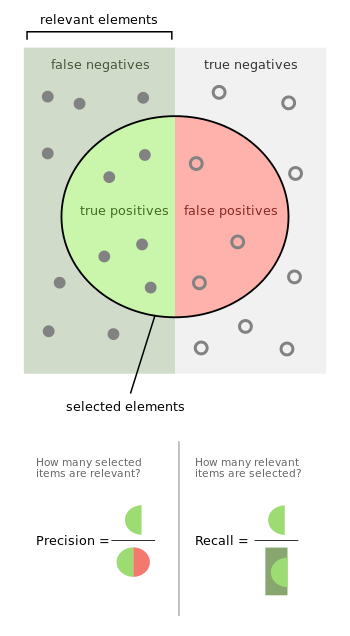
\includegraphics[width=7cm]{./immagini/precisionrecall.png}
    \caption{\href{https://upload.wikimedia.org/wikipedia/commons/2/26/Precisionrecall.svg}{Definizione grafica di precision e recall, fonte: Wikipedia}}
    \label{precision recall}
\end{figure}
\FloatBarrier
Vengono definiti due parametri per la scelta di $\alpha$:
\begin{itemize}
    \item \textbf{Precision}: rappresenta quanti veri positivi sono stati rilevati su un totale composto da veri positivi e falsi positivi.
    \item \textbf{Recall}: rappresenta il numero effettivo di elementi positivi che sono stati rilevati su un totale di falsi negativi e veri positivi.
\end{itemize}
In particolare, nel caso in esame:
\begin{itemize}
    \item per vero positivo si intende una coppia di password simili correttamente rilevate come tali;
    \item per falso positivo si intende una coppia di password diverse erroneamente rilevate come simili;
    \item per falso negativo si intende una coppia di password simili erroneamente non rilevate come tali.
\end{itemize}
Un valore di precision basso implica una imprecisa distinzione tra password simili e password non simili; un valore di recall basso invece comporta avere molte password simili non rilevate come tali.

Nel paper di riferimento di Bijeeta et alii~\cite{bijeeta} viene considerato un valore di recall molto alto (99\%) e una percentuale di precision nettamente più bassa (60\%). Per questo motivo $\alpha$ è stato posto a $0.5$.

\begin{figure}[h]
    \centering
    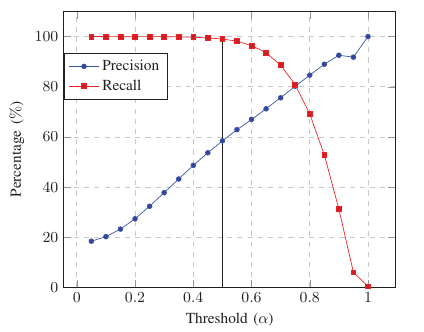
\includegraphics[width=11cm]{./immagini/precision_recall_paper_bijeeta.png}
    \label{precisionbijeeta}
    \caption{Precision e recall di Bijeeta et al.~\cite{bijeeta}}
\end{figure}
\subsection{Modelli compressi di word embedding}
\label{sec:modelli compressi word embedding}
Il modello prodotto da Bijeeta et alii~\cite{bijeeta} è stato successivamente compresso, in modo da ridurre la dimensione da 1.5 GB a 3 MB, senza che la qualità delle performance venisse ridotta, mediante tecniche di quantizzazione.
Per la produzione del modello compresso si è tenuto conto del parametro $\eta$ che determina il rapporto di compressione. Per la valutazione della compressione, sono stati prodotti più modelli in base a differenti valori $\eta$; infine è stato scelto il modello con $\eta=5$ e dimensione complessiva di 3 MB, poiché il valore di recall non ha subito notevoli variazioni.
\begin{figure}[h]
    \centering
    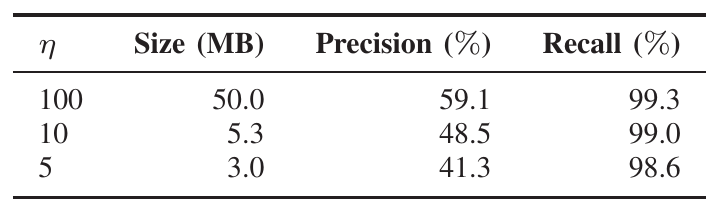
\includegraphics[width=9cm]{./immagini/compressed_model.png}
    \label{compressed_model}
    \caption{Precision e recall in base al rapporto di compressione $\eta$ del modello di Bijeeta et alii~\cite{bijeeta}}
\end{figure}
\section{Modifiche e analisi del progetto}
\label{sec:modifiche analisi del progetto}
Per questo progetto sono state effettuate diverse scelte:

\begin{itemize}
    \item Si è scelto di non implementare pass2path, per motivi di complessità e di costo in termini di testing;
    \item sono stati modificati i criteri di filtraggio del dataset per allenare il modello di word embedding;
    \item sono state utilizzate euristiche diverse rispetto a pass2path;
    \item sono stati modificati i parametri per allenare la rete neurale che ricava la similarità tra password.
\end{itemize}

\chapter{Implementazione}
\label{ch:implementazione}

Lo scopo del progetto è sviluppare un classificatore che, date due password, determini se sono simili tra loro (e quindi potenzialmente non sicure) o meno.

A tal proposito sono stati implementati modelli di word embedding, i quali permettono di rappresentare parole in uno spazio vettoriale preservando proprietà semantiche quali la similarità e la co-occorrenza nel medesimo contesto.
Come modello è stato scelto FastText, il quale sfrutta informazioni sugli n-gram della parola per determinarne l'embedding~\cite{biijeta}.

Si è deciso di allenare 5 diversi modelli:
\begin{itemize}
    \item Il modello di Bijeeta et alii~\cite{biijeta} che utilizza la libreria \texttt{word2keypress} per ricavare la sequenza di tasti premuti per specifici caratteri, numero minimo di n-gram pari a 1, e numero di epoche per allenare la rete pari a 5.
    \item Un modello che utilizza \texttt{word2keypress}, con numero minimo di n-gram pari a 2, e numero di epoche per allenare la rete pari a 10.
    \item Tre modelli che non rilevano la sequenza di tasti premuti:
    \begin{itemize}
        \item Uno con numero minimo di n-gram pari a 1, e numero di epoche per allenare la rete pari a 5.
        \item Uno con numero minimo di n-gram pari a 2, e numero di epoche per allenare la rete pari a 5.
        \item Uno con numero minimo di n-gram pari a 2, e numero di epoche per allenare la rete pari a 10.
    \end{itemize}
\end{itemize}

\section{Precondizioni}
Prima della fase di allenamento della rete, è necessario avere un dataset valido di password; nel progetto è stato utilizzato lo stesso data breach da 45 GB citato da Bijeeta et alii~\cite{biijeta}, tuttavia sono stati scelti criteri diversi di filtraggio:
\begin{itemize}
    \item Sono state rimossi gli account con password con lunghezza inferiore a 4 caratteri o maggiore di 30.
    \item Sono state rimosse gli account con password che presentavano caratteri non ASCII o non stampabili.
    \item Sono stati rimossi gli account creati da bot, riconoscibili grazie al numero di occorrenze della stessa email nel dataset, superiore a 100.
    \item Sono stati rimossi gli account con password contententi sequenze esadecimali (identificate da \texttt{\$HEX[]} e \texttt{\textbackslash x}).
    \item Sono stati rimossi sequenze che rappresentano caratteri in HTML, come:
    \begin{itemize}
        \item \texttt{\&gt} (simbolo $>$);
        \item \texttt{\&ge} (simbolo $\geq$);
        \item \texttt{\&lt} (simbolo $<$)
        \item \texttt{\&le} (simbolo $\leq$);
        \item \texttt{\&\#} (ovvero i codici di entità in HTML);
        \item \texttt{amp}.
    \end{itemize}
    \item Sono stati rimossi gli account che presentavano meno di 2 password, poiché più password per utente risultano indispensabili per ricavare la similarità.
\end{itemize}
Successivamente, in accordo con Bijeeta et alii~\cite{biijeta}, per i modelli che prevedevano la memorizzazione delle sequenze di tasti premuti, è stata utilizzata la libreria python \href{https://github.com/rchatterjee/word2keypress}{\texttt{word2keypress}}.
Successivamente i risultati sono stati salvati in un file \texttt{csv} nel seguente formato:
\begin{center}
    \texttt{sample@gmail.com: ["'97314348'", "'voyager<s>1'"]}
\end{center}

\section{Impostazioni dell'ambiente}
Per potere allenare il modello è stato utilizzato \texttt{gensim.FastText}~\cite{gensim}.
\\
\texttt{gensim} è una libreria python multipiattaforma e open source che racchiude un'ampia scelta di modelli di word embedding pre allenati~\cite{gensim}.
Per estrapolare i dati dal file \texttt{csv} è stata sviluppata una classe ausiliaria \texttt{PasswordRetriever}.
\section{Allenamento del modello}
\subsection{Parametri di FastText}
\begin{minted}[
    frame=lines,
    framesep=2mm,
    baselinestretch=1.2,
    bgcolor=LightGray,
    fontsize=\footnotesize,
    linenos
    ]{python}
negative = 5
subsampling = 1e-3
min_count = 10
min_n = 2
max_n = 4
SIZE = 200
sg = 1
\end{minted}
Per questo progetto è stato utilizzato il modello \emph{Skip-gram} (\texttt{sg = 1}) e il negative sampling~\cite{negative}:
\begin{itemize}
    \item Il modello Skip-gram (parametro \texttt{sg = 1}) è stato scelto in quanto la rappresentazione distribuita dell'input è stata utilizzata per prevedere il contesto delle password. In particolare, risulta efficace per determinare quali caratteri intorno a una specifica sequenza sono presenti; in questo modo il modello riesce a imparare password non presenti nel corpus fornito per l'allenamento.~\cite{fasttext}
    \item Il negative sampling (parametro \texttt{negative = 5}) rende l'allenamento più veloce, poiché ciascuna sezione dell'allenamento aggiorna solo una piccola percentuale dei pesi del modello.~\cite{negative} Per dataset di dimensioni maggiori (come in questo caso) è consigliabile impostare il suo valore tra 2 e 5.~\cite{gensim}
    \item La dimensione del vettore contenente gli embedding è impostato a $200$ (parametro \texttt{SIZE = 200}), in modo da potere allenare più velocemente il modello. Normalmente viene raccomandata una dimensione pari a \texttt{SIZE = 300}.~\cite{gensim}
    \item Il subsampling ignora le password più frequenti, ovvero che presentano più di 1000 occorrenze.
    \item \texttt{mincount} rappresenta il numero minimo di occorrenze di una password nel dataset di training affinché venga considerata nell'allenamento~\cite{biijeta}~\cite{gensim}.
    \item \texttt{min\_n} e \texttt{max\_n} rappresentano rispettivamente il numero minimo e massimo degli n-gram. Gli N-gram vengono utilizzati per prevedere una sequenza di caratteri e il contesto di quest'ultima. In questo caso essi rappresentano una sequenza di caratteri contigui e il loro scopo è di dare informazioni di contesto e posizionali di una determinata sequenza all'interno di una password~\cite{biijeta}~\cite{gensim}.
\end{itemize}

\subsection{Allenare FastText}
La lista di password relativa a ciascun utente (\texttt{password\_list}) viene ottenuta grazie alla classe ausiliaria \texttt{PasswordRetriever}. Il modello di FastText si basa su \texttt{password\_list} e viene allenato con i parametri elencati precedentemente.

\begin{minted}[
    frame=lines,
    framesep=2mm,
    baselinestretch=1.2,
    bgcolor=LightGray,
    fontsize=\footnotesize,
    linenos
    ]{python}
filename='../train.csv'
password_list = PasswordRetriever(filename)
trained_model = FastText(password_list, size=SIZE, min_count=min_count,
                        workers=12, negative=negative,
                        sample=subsampling, window=20,
                        min_n=min_n, max_n=max_n)
\end{minted}

\section{Compressione del modello}
Il modello allenato ha un peso complessivo pari a 4.8 GB, e ciò comporta i seguenti problemi:
\begin{itemize}
    \item Meno efficiente in termini di spazio, di conseguenza l'utilizzo del modello è limitato su sistemi con vincoli di memoria o di spazio.
    \item È difficile utilizzare il modello in contesti distribuiti, poiché non è facilmente trasportabile.
\end{itemize}
Per comprimere il modello si è utilizzata la libreria \texttt{compress\_fasttext}, che sfrutta tecniche di quantizzazione e di feature selection.~\cite{compress-fasttext}
\begin{minted}[
    frame=lines,
    framesep=2mm,
    baselinestretch=1.2,
    bgcolor=LightGray,
    fontsize=\footnotesize,
    linenos
    ]{python}
big_model = gensim.models.fasttext.load_facebook_vectors('model.bin')
small_model = compress_fasttext.prune_ft_freq(big_model, pq=True)
small_model.save('compressed_model')
\end{minted}

Viene definito come \emph{feature selection} il processo di selezione delle feature più importanti da usare per costruire un modello~\cite{bishop2006pattern}~\cite{feature}.

Per \emph{Product quantization} si intende un particolare tipo di quantizzazione vettoriale, che viene utilizzata per la compressione di modelli di linguaggio naturale e di elaborazione di immagini e consente di generare in modo non esponenziale una quantità grande di codice in tempi contenuti e con costi ridotti in termini di memoria~\cite{biijeta}~\cite{compress-fasttext}~\cite{quantization}.

Il modello compresso ottenuto dalle operazioni di quantizzazione e di feature selection ha una dimensione di 20 MB.
\chapter{Risultati}
\section{Differenze tra modello normale e compresso}
Dati i problemi che comportavano l'utilizzo dei modelli da 4.8 GB, si è scelto di utilizzare per l'analisi dei risultati le versioni compresse da appena 20 MB ottenute tramite product quantization.
Per misurare la differenza di prestazioni tra il modello originale e la sua versione compressa si è considerato come riferimento il modello di Biijeta et alii, avente le seguenti caratteristiche:
\begin{itemize}
    \item traduzione della sequenza dei tasti premuti con \texttt{word2keypress}
    \item numero minimo di n-gram pari a 1;
    \item numero di epoche di training pari a 5.
\end{itemize}

Per entrambi i modelli si è tenuto conto del valore di precision e recall, in modo da fornire una valutazione efficace del modello.
Sono state osservate differenze minime riguardanti i valori, motivo per il quale si è scelto di considerare soltanto le versioni compresse per valutare gli altri modelli.

\section{Euristiche adottate}
\subsection{Ground truth e prediction}
Ground truth: cosa è
Prediction: cosa è
euristica.

\section{Similarità: un confronto}
\section{Criticità del modello proposto da Bijeeta et alii}
\section{Rappresentazione grafica della distanza tra parole}

\label{ch:risultati}



% Conclusioni
\chapter*{Conclusioni}
\chaptermark{Conclusioni}
\addcontentsline{toc}{chapter}{Conclusioni}
In questo progetto di tesi ci si è soffermati sul problema dell'utilizzo di varianti di password precedenti e di possibili approcci di prevenzione. Per potere comprendere quali siano le varianti ci si è soffermati non solo sulla forma delle password, ma anche sulla sfera semantica che ricoprono, grazie a tecniche di word embedding, che consentono la traduzione di parole in vettori di numeri reali. A tal scopo è stato utilizzato \texttt{gensim.FastText} come modello di word embedding per potere fornire un punteggio di similarità tra due password, il cui apprendimento è influenzato dall'insieme di \texttt{n-gram} di una parola.

Prima dell'allenamento di FastText, è stato filtrato un dataset da 43 GB, escludendo gli utenti con meno di due password; successivamente si è diviso il dataset in training set e test set e si è deciso di allenare 5 modelli e di confrontarli tra loro, in base ai seguenti fattori:
\begin{itemize}
    \item Conversione mediante libreria \texttt{word2keypress} delle password in sequenza di tasti premuti per ottenere caratteri maiuscoli e caratteri speciali.
    \item Numero minimo di n-gram, ovvero la lunghezza minima della sequenza di caratteri che compone in parte la password.
    \item Numero di epoche con cui è stato allenato il modello.
\end{itemize}
Dopodiché, grazie al metodo di \texttt{product quantization}, è stato compresso il modello, in modo da ridurre la dimensione da 4.8 GB a 20 MB, senza subire perdita di qualità. In seguito, è stata scelta un'euristica che, per la valutazione della similarità di due password, effettuasse i seguenti controlli:
\begin{itemize}
    \item verifica della password con la variante maiuscola;
    \item verifica della password con la variante minuscola;
    \item verifica della password con la traduzione in codice \texttt{l33t};
    \item verifica se l'edit distance della password superasse 5.
\end{itemize}
Infine è stato ricavato il grafico di precision e recall, utile per potere fornire una valutazione dei modelli e della loro affidabilità, ed è stato scoperto che il modello implementato dal paper di riferimento di Bijeeta et alii~\cite{bijeeta} che utilizza l'euristica precedentemente citata risulta il peggiore in termini di performance. Ciò era dovuto alla traduzione da parte di \texttt{word2keypress} di caratteri in sequenze composte da \texttt{<c> <s>}, comuni a più password che utilizzavano una alternanza di maiuscole e caratteri speciali.

Un altro problema del modello precedentemente citato era determinato dal numero minimo di n-gram, pari a 1, che risultava troppo dispersivo per potere consentire un apprendimento efficace da parte del modello dei caratteri che componevano una password.

Per risolvere, si è deciso di allenare un modello, che non tenesse conto della sequenza di tasti premuti e che, in fase di apprendimento, dalla durata di 5 epoche, considerasse un numero minimo di n-gram pari a 2.

Quest'ultimo è risultato il migliore tra tutti i modelli allenati.

\section{Sviluppi futuri}
\label{sec:sviluppi futuri}
Sono possibili diversi utilizzi del modello ottenuto in questo progetto:
\begin{itemize}
    \item In un ambiente distribuito dedicato al cambio di password, dove l'utente possa fornire la vecchia password e la nuova. Il modello compresso può determinare se la nuova password possa essere considerata abbastanza sicura rispetto a quella vecchia, e può essere inviato come payload JavaScript, mentre il controllo di sicurezza può essere effettuato lato client, assicurandosi che la nuova candidata password non venga inoltrata a un server remoto, prima di diventare definitiva.
    Un vantaggio nell'utilizzare i modelli compressi risulta nel garantire l'anonimizzazione delle password, poiché esse vengono rappresentate come word embedding, e non sono reversibili, pertanto in fase di intercettazione non comportano alcun rischio. Successivamente il server può effettuare un controllo sul database per vedere se la password risulta sicura rispetto alla versione precedente. Questo comporta non dovere salvare in un database le password in chiaro e non dovere ricorrere ad algoritmi di crittografia, grazie alle proprietà dei word embedding.
    \item Confronto con il modello che sfrutta i bloom filter, per poi stabilire quale approccio sia il migliore.
\end{itemize}


% Ringraziamenti
\chapter*{Ringraziamenti}
\chaptermark{Ringraziamenti}
\addcontentsline{toc}{chapter}{Ringraziamenti}
Ringrazio i miei relatori per il supporto e per avermi dato l'opportunità di approfondire questa tema.

Altrettanto ringrazio i miei genitori e tutti coloro che mi sono stati vicini in questo percorso e hanno creduto in me. A loro è dedicata questa tesi.

% Bibliografia
%\chapter*{Bibliografia}
\chaptermark{Bibliografia}
\addcontentsline{toc}{chapter}{Bibliografia}

\section*{Libri}
\begingroup
\let\clearpage\relax
\printbibliography[category=libri,heading=none]
\endgroup

\section*{Articoli}
\begingroup
\let\clearpage\relax
\printbibliography[category=articoli,heading=none]
\endgroup

\section*{API}
\begingroup
\let\clearpage\relax
\printbibliography[category=api,heading=none]
\endgroup

\section*{Immagini}
\begingroup
\let\clearpage\relax
\printbibliography[category=immagini,heading=none]
\endgroup
\phantomsection
\printbibliography[heading=bibintoc]

\end{document}
